\documentclass{sig-alternate}


\usepackage[latin1]{inputenc}
\usepackage{amssymb}
\setcounter{tocdepth}{3}
\usepackage{graphicx}
\usepackage{subfigure}

\usepackage{url}

\begin{document}

\title{Modeling browser-based distributed evolutionary computation systems} 

\numberofauthors{1} %  in this sample file, there are a *total*
% of EIGHT authors. SIX appear on the 'first-page' (for formatting
% reasons) and the remaining two appear in the \additionalauthors section.
%
\author{
% You can go ahead and credit any number of authors here,
% e.g. one 'row of three' or two rows (consisting of one row of three
% and a second row of one, two or three).
%
% The command \alignauthor (no curly braces needed) should
% precede each author name, affiliation/snail-mail address and
% e-mail address. Additionally, tag each line of
% affiliation/address with \affaddr, and tag the
% e-mail address with \email.
%
% 1st. author
\alignauthor
Som E. One\\
       \affaddr{Some Institute}\\
       \email{em@a.il}
}


\maketitle

\begin{abstract}
From the era of big science we are back to the "do it yourself", where
you do not have any money to buy clusters or subscribe to grids but
still have algorithms that crave many computing nodes and need them to
measure scalability. Fortunately, this coincides with the era of big
data, cloud computing, and browsers that include JavaScript virtual
machines. Those are the reasons why this paper will focus on two
different aspects of volunteer or freeriding computing: first, the
pragmatic: where to find those resources, which ones can be used, what
kind of support you have to give them; and then, the theoretical: how
evolutionary algorithms can be adapted to a environment in which nodes
come and go, have different computing capabilities and operate in
complete asynchrony of each other. We will examine the setup needed to
create a very simple distributed evolutionary algorithm using
JavaScript and then find a model of how users react to it by
collecting data from several experiments featuring different classical
benchmark functions. 
\end{abstract}

\keywords{Evolutionary computation, volunteer computing, distributed
  computing, node.js, javascript}

\section{Introduction}

The world has computational resources in spades. Most of them do not
belong to you or your lab. That does not mean you cannot use it. The
problem is how. 

Most theory in parallel computing has been devoted to predict and
optimize the performance in systems where the number of nodes, their
connections, and the time every one is devoting to the computation is
known in advance. However, even if Big Science is not really over and
it is slated to come back, the era of
Citizen Science already started a few years ago (with SETI@home \cite{david-seti:home} and then BOINC \cite{boinc_grid04}) and it
offers a vast amount of computational resources to attract, if only
you know how. But there is a challenge: knowing, or at least having a
ballpark, of how your algorithm is going to perform in this uncertain
environment, where none of the factors is known: neither the number of
nodes, through how they are connected, to how long are they going to
be focused on doing what you want them to. That is why some effort is
needed to first understand the dynamics of the decision to participate
in an experiment that requires you to click on a link and then stay
for a while looking at the screen (or just leave it there running).

Besides, since Amazon started selling EC2 several years ago, reliable
and scalable computing resources are also available for a low price
and on demand. Recently, Google has also refurbished its offering
lowering their prices. This means that the conjunction of free or
low-cost cloud computing engines, volunteer computing systems and and
untapped capability of desktop systems can be used for creating
massive, or at least potentially massive, distributed computing
experiments. 

The rest of the paper is organized as follows: next we will present
the state of the art in volunteer computing and its modelization. We
will proceed to describe the experimental setup in Section
\ref{sec:exp}, some preliminary results in Section \ref{sec:res} and
finally we will present our conclusions in Section \ref{sec:conc}
along with future lines of work. 

\section{State of the art}
\label{sec:soa}

Using the web as a resource for distributed, or plainly user based,
evolutionary computation has a long history since JavaScript was
introduced as a browser-based language in 1997 and even before, when
other procedures, including Flash animations, VBScript, ActiveX or Java applets were
used. Java was pointed out in \cite{soares1998get} as a ``language for
internet'' and
\begin{quote}
Java can bring some important advantages... solves architectural
heterogeneity [...] easy to install and [...] built-in security
mechanisms
\end{quote}
The same paper by Soares et al. describes JET, a system that supports
the execution of parallel applications over the Internet. In fact the
same paper describes some other systems working at the same time,
except they cannot be used for science since they do not have a
comprehensive statistics support like JET. 

However, Java (and all the other technologies) is not universal in the
sense than an extra component, namely, the Java virtual machine, has
to be installed in the browser. JavaScript
\cite{flanagan2006javascript} was introduced in 1997 as a
browser-embedded language and has, since them, become a set of standards
\cite{ECMA-262} for the language, its components and future versions
that have been widely adopted by the industry and also by scientists,
who used them for creating a non-distributed evolutionary algorithm on
the browser as early as 1998 \cite{jj-ppsn98}. 

The potential for volunteer computing using browsers was realized
later on \cite{sarmenta-bayanihan} as well as the potential for
mischief of users with code in their hands
\cite{sarmenta-sabotagetolerance} however, these early efforts by
Sarmenta once again used Java and not JavaScript, making this effort
less universal. JavaScript can be used either for unwitting
\cite{unwitting-ec} or volunteer
\cite{langdon:2005:metas,gecco07:workshop:dcor} distributed
evolutionary computation and has been used ever since by several
authors, including recent efforts \cite{duda2013distributed} that even
used the client's GPU \cite{duda2013gpu}.

There have been relatively few efforts to analyze what is the
performance that can be obtained from these volunteer computing
effort. There was some effort initially to dodge the issue by making
the algorithm adaptive to the kind of resources allotted to it
\cite{sarmenta-bayanihan}, which is actually not such a big problem in
algorithms such as the evolutionary algorithm that can easily be
paralelized via population splitting or farming out evaluations to all
the nodes available. 

\section{Methodology}
\label{sec:exp}

\begin{figure*}[h!tb]
  \centering
  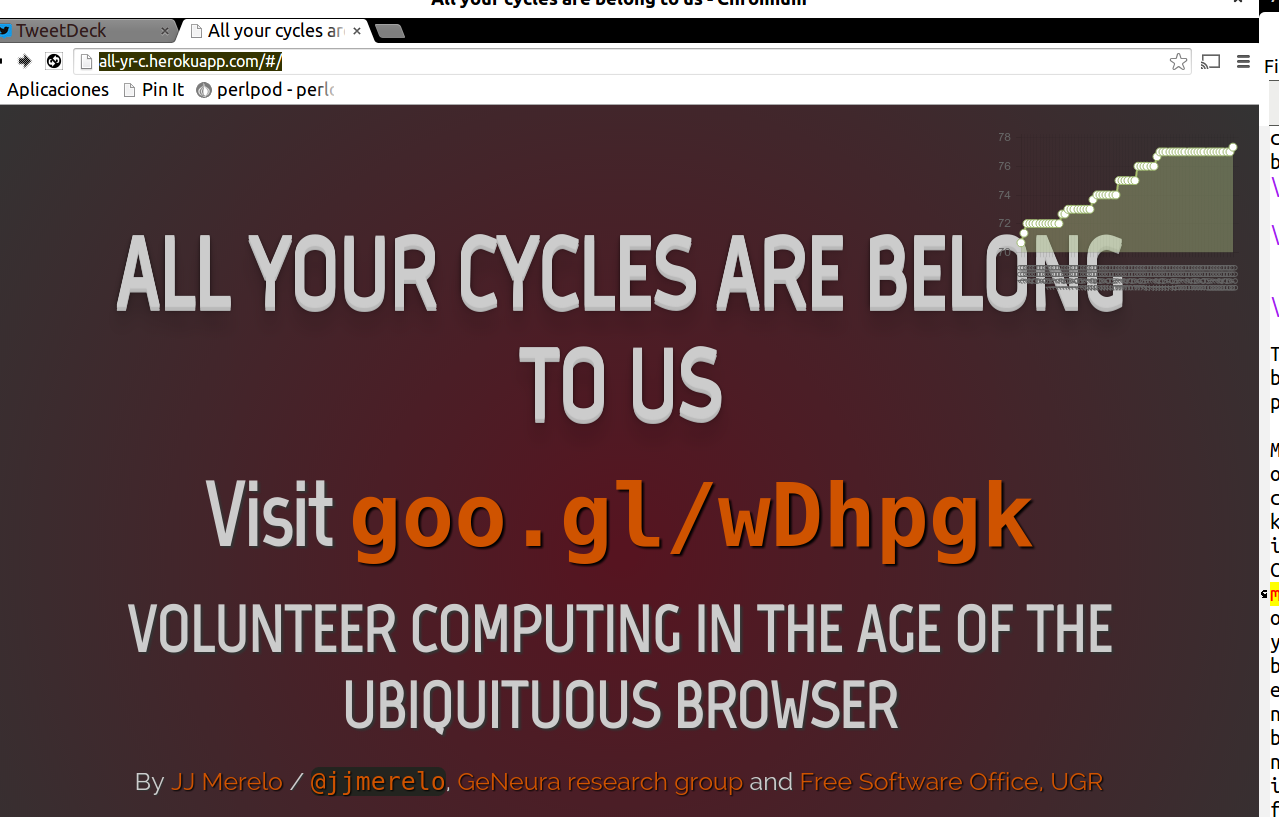
\includegraphics[trim=0cm 2cm 0cm 3cm, width=10cm]{img/screenshot.png}
  \label{fig:sshot}
  \caption{Screenshot of the talk that includes at the graph
    that shows the progression of the evolutionary
    algorithm at the top right corner}
\end{figure*}


\section{Conclusion}

In this paper we will offer our experience on using browser-based computing since 1999 \cite{jesusIWANN99} and other emerging paradigms, such as peer to peer based computing \cite{evag:gpem}, mainly applied to the design of evolutionary algorithms. 

There are many issues involved in using these resources: from adapting current algorithms so that they match this environment \cite{agajaj} to check which EA configuration works the best in it, or creating a framework that can use it easily \cite{nodeo2014}. But the main challenge is that asking people to contribute resources implies that you are opening your science to society and you have to give something in return: you have to adopt a set of best practices that have come to be known as Open Science, because ``Give, and it shall be given unto you'', you will get as much back from society as you give to it opening your science and explaining it to the public. This, among other things, means that popularity will become directly performance of the metacomputer you create by attracting more users.


\bibliographystyle{abbrv}
\bibliography{geneura,volunteer,javascript,ror-js}

\end{document}
